\documentclass[conference]{IEEEtran}
\IEEEoverridecommandlockouts

\usepackage{cite}
\usepackage{amsmath,amssymb,amsfonts}
\usepackage{algorithmic}
\usepackage{graphicx}
\usepackage{textcomp}
\usepackage{xcolor}
\usepackage{url}
\usepackage{array}
\usepackage{booktabs}
\usepackage{tabularx} % Added for automatic column width calculation
\usepackage{tikz}
\usetikzlibrary{arrows.meta,positioning,shapes.geometric}
\newcolumntype{Y}{>{\centering\arraybackslash}X}
\newcolumntype{P}[1]{>{\centering\arraybackslash}p{#1}}
\setlength{\tabcolsep}{4pt}
\renewcommand{\arraystretch}{1.2}

\def\BibTeX{{\rm B\kern-.05em{\sc i\kern-.025em b}\kern-.08em
    T\kern-.1667em\lower.7ex\hbox{E}\kern-.125emX}}

\begin{document}

\title{Resource-Aware Adaptive Scheduling for Online Code Judge Systems: From Bare-Metal Calibration to Hyperscale Cloud Provisioning}

\author{
\IEEEauthorblockN{Bharath Aashish R}
\IEEEauthorblockA{\textit{Dept. of Computer Science \& Engineering} \\
\textit{Easwari Engineering College}\\
Chennai, India \\
bharathaashish@gmail.com}
\and
\IEEEauthorblockN{Dhanush M}
\IEEEauthorblockA{\textit{Dept. of Computer Science \& Engineering} \\
\textit{Easwari Engineering College}\\
Chennai, India \\
dhanush.m.0808@gmail.com}
\and
\IEEEauthorblockN{Hemanthkumar K}
\IEEEauthorblockA{\textit{Dept. of Computer Science \& Engineering} \\
\textit{Easwari Engineering College}\\
Chennai, India \\
hemanthkumar2k04@gmail.com}
\and
\IEEEauthorblockN{Iniyaa P}
\IEEEauthorblockA{\textit{Dept. of Computer Science \& Engineering} \\
\textit{Easwari Engineering College}\\
Chennai, India \\
iniyaapaari@gmail.com}
\and
\IEEEauthorblockN{Mrs. Indumathy P}
\IEEEauthorblockA{\textit{Assistant Professor, Dept. of CSE} \\
\textit{Easwari Engineering College}\\
Chennai, India \\
indumathy.p@eec.srmrmp.edu.in}
}

\maketitle

\begin{abstract}
Online Code Judge (OJ) systems often assign every submission a fixed worst-case resource limit, such as 2048~MiB of RAM and 2.0 CPU cores. Our measurements show substantial underutilization: among 69 accepted submissions running at the 256~MiB tier, 76.8\% used less than 25~MiB of resident set size (RSS), with a median of 13.4~MiB. We present RAAS-OCJS, a resource-aware scheduling framework that combines Linux cgroups~v2 with tiered allocation and AST-based XGBoost routing. Kernel-level profiles from C++, Python, Java, and C programs were used to drive a 10,000-submission contest simulation. Compared with static allocation, the adaptive scheme reduced reserved RAM by 47.22\% and CPU core-hours by 22.09\%. In a simulated 500-submission freeze rush, queue wait decreased from 12,386.2~ms to 0.0~ms, while P95 turnaround decreased from 24,918.4~ms to 1,186.8~ms. A 128~MiB boundary experiment additionally isolates three independent failure modes, which together establish 256~MiB as the practical minimum tier. These results support adaptive resource allocation for improving judge-system utilization and concurrency.
\end{abstract}

\begin{IEEEkeywords}
Online judge systems, resource-aware scheduling, adaptive cgroups, soft watermark, AST analysis, XGBoost, cloud provisioning, queue latency.
\end{IEEEkeywords}

\section{Introduction}
Online code judge (OJ) platforms underpin computer science education, competitive programming contests (such as the International Collegiate Programming Contest, ICPC), and automated technical interviews \cite{wasik2018survey}. As programming education expands, judges must evaluate thousands of code submissions concurrently while guaranteeing deterministic isolation and strict sandboxing. Existing research has addressed this computational demand primarily through infrastructure-level expansion: deploying elastic cloud clusters \cite{pan2022cloud}, distributing jobs over message queues \cite{song2025idl}, or deploying geographically replicated edge judges \cite{wang2021metaoj}.

These approaches share a fundamental, costly assumption: \textit{every submission, regardless of its computational structure, receives identical, worst-case sandbox resource ceilings} (typically 2048~MiB of RAM and 2.0 CPU cores).

This convention creates three practical problems:
\begin{itemize}
    \item \textbf{Resource Underutilization}: Most contest submissions implement standard algorithmic logic (e.g., prefix sums, two pointers, greedy string scans), and in our measurements these typically required 5~MiB to 25~MiB of resident set size (RSS), with 76.8\% of accepted runs below 25~MiB and a median of 13.4~MiB (Table~\ref{tab:mem_dist}). Reserving 2048~MiB for each of them leaves most of that allocation idle.
    \item \textbf{Concurrency Starvation on Fixed Hardware}: In air-gapped regional contests or campus lab servers, where external cloud bursting is not an option, the judge runs on a fixed physical machine (e.g., 15~GiB usable RAM). A static 2048~MiB quota limits concurrency to 7 execution slots on that host, which produces queue backlogs and submission timeouts during a scoreboard freeze rush.
    \item \textbf{Cloud Billing Inflation}: Public cloud providers (AWS, GCP, Azure) bill by reserved node capacity, not actual usage. Provisioning for the worst case means contest organizers end up renting far more virtual machines than the workload actually needs: our projection in Section~V estimates 36 instances where 5 suffice, a 7.2$\times$ over-provisioning.
\end{itemize}

To address this, this paper presents \textbf{RAAS-OCJS} (Resource-Aware Adaptive Scheduling for Online Contest Judge Systems), which introduces a two-tier execution framework:
\begin{enumerate}
    \item A lightweight default sandbox (\textbf{Tier 1: 256~MiB RAM, 1.0 CPU core}) that completed 30 of the 38 light-tier submissions in our 72-run benchmark (78.9\%) without ever needing promotion, and 80.4\% of submissions in the simulated contest;
    \item An active Linux cgroup~v2 soft watermark ($\theta = 70\%$, corresponding to 179.2~MiB) that detects high memory utilization in-flight and lifts the container's memory and CPU limits to \emph{uncapped} mid-execution, without restarting the container or losing process state. Measured from submission acceptance to completed promotion this takes 248--808~ms depending on the language runtime;
    \item An offline Machine Learning (XGBoost) classifier driven by Tree-sitter Abstract Syntax Tree (AST) static structural metrics that predicts memory-intensive jobs upon ingress.
\end{enumerate}



\section{Theoretical Model and Queueing Architecture}

\subsection{Mathematical Formulation of Memory Waste}
Let $S = \{s_1, s_2, \dots, s_N\}$ denote a sequence of $N$ submissions entering an online judge. Under static overprovisioning, the system assigns a fixed resource allocation:
\begin{equation}
R_{\mathrm{alloc}}(s_i) = R_{\mathrm{max}}, \quad \forall s_i \in S
\end{equation}
where $R_{\mathrm{max}}$ is typically 2048~MiB. Let $R_{\mathrm{peak}}(s_i)$ denote the actual peak resident set size (RSS) consumed by $s_i$. The unallocated, wasted memory for submission $s_i$ is:
\begin{equation}
\mathrm{Waste}(s_i) = R_{\mathrm{alloc}}(s_i) - R_{\mathrm{peak}}(s_i)
\end{equation}
The system-wide memory waste percentage $W$ across a contest of $N$ submissions is:
\begin{equation}
W = \left[ \frac{\sum_{i=1}^N \left( R_{\mathrm{alloc}}(s_i) - R_{\mathrm{peak}}(s_i) \right)}{\sum_{i=1}^N R_{\mathrm{alloc}}(s_i)} \right] \times 100\%
\end{equation}
Because introductory and greedy problems require merely 6~MiB to 25~MiB, $R_{\mathrm{peak}}(s_i) \ll R_{\mathrm{max}}$. Our simulation of this waste model reports 97.47\% of allocated memory wasted under the static baseline.

\subsection{Concurrency Capacity and Queueing Collapse}
On a host with usable physical RAM $M_{\mathrm{host}}$ and operating system reserve $M_{\mathrm{os}}$, the safe concurrency capacity $K$ under non-overcommitted execution is:
\begin{equation}
K_{\mathrm{safe}} = \left\lfloor \frac{M_{\mathrm{host}} - M_{\mathrm{os}}}{R_{\mathrm{alloc}}} \right\rfloor
\end{equation}
On our 15~GiB physical calibration host ($M_{\mathrm{host}} = 15,360$~MiB, $M_{\mathrm{os}} = 1,024$~MiB), baseline static allocation ($R_{\mathrm{max}} = 2048$~MiB) limits concurrency strictly to:
\begin{equation}
K_{\mathrm{safe, baseline}} = \left\lfloor \frac{15,360 - 1,024}{2048} \right\rfloor = 7 \text{ slots}
\end{equation}

We model contest submission arrival as a non-homogeneous Poisson process with time-varying arrival rate $\lambda(t)$. Service times follow a general distribution with mean $E[X] = 1/\mu$ and variance $\sigma^2$, constituting an $M/G/K$ queueing system.

During a freeze rush spike of 500 submissions in 30~s ($\lambda = 16.67$~submissions/s), against average service time $E[X] \approx 0.85$~s, the 7-slot baseline service capacity is $\mu = 7 / 0.85 \approx 8.24$~submissions/s. Because $\lambda > \mu$, queue backlogs explode immediately. Under RAAS-OCJS with $R_{\mathrm{light}} = 256$~MiB, concurrency expands safely to $\lfloor 14{,}336/256 \rfloor = 56$ slots (utilizing 93.3\% of host RAM as reserved capacity, which the watermark then releases in practice). At $K = 56$, $\mu = 56 / 0.85 \approx 65.88$~submissions/s, satisfying $\mu \gg \lambda$ and maintaining zero queue wait ($L_q \approx 0$).

\subsection{Dynamic Soft Watermark Governance}
RAAS-OCJS implements a two-tier scheduling policy:
\begin{itemize}
    \item \textbf{Tier 1 (Light Sandbox)}: $R_{\mathrm{light}} = 256$~MiB, 1.0 CPU core (1024 CFS shares).
    \item \textbf{Tier 2 (High Sandbox)}: unbounded, 2.0 CPU cores (2048 CFS shares). The 2048~MiB figure is the \emph{static baseline's} convention that we compare against, not a ceiling RAAS-OCJS re-imposes after promotion.
\end{itemize}
Rather than statically placing containers into Tier 2, all submissions enter Tier 1 by default. The judge daemon configures the Linux cgroups v2 controller with a soft memory watermark threshold $\theta = 0.70$:
\begin{equation}
\mathrm{Threshold}_{\mathrm{wm}} = \theta \times R_{\mathrm{light}} = 0.70 \times 256\text{ MiB} = 179.2\text{ MiB}
\end{equation}
When $R_{\mathrm{current}}(t) \ge \mathrm{Threshold}_{\mathrm{wm}}$, the kernel emits a pressure notification. The judge daemon then lifts the limits in parallel with process execution, issuing \texttt{docker update --memory 0 --cpus 0} to raise both the memory ceiling and the CPU quota to uncapped. This leaves a 76.8~MiB safety cushion ($256 - 179.2$) so the update can complete before an OOM condition occurs. Promotion targets \emph{uncapped} rather than a fixed 2048~MiB tier: the watermark fires precisely when a submission has already shown that it outgrows Tier~1, and measured demand for such submissions ranged from 200~MB to 254~MB, so no single fixed ceiling is appropriate.

% System architecture overview
\begin{figure*}[!t]
\centering
\resizebox{0.86\textwidth}{!}{%
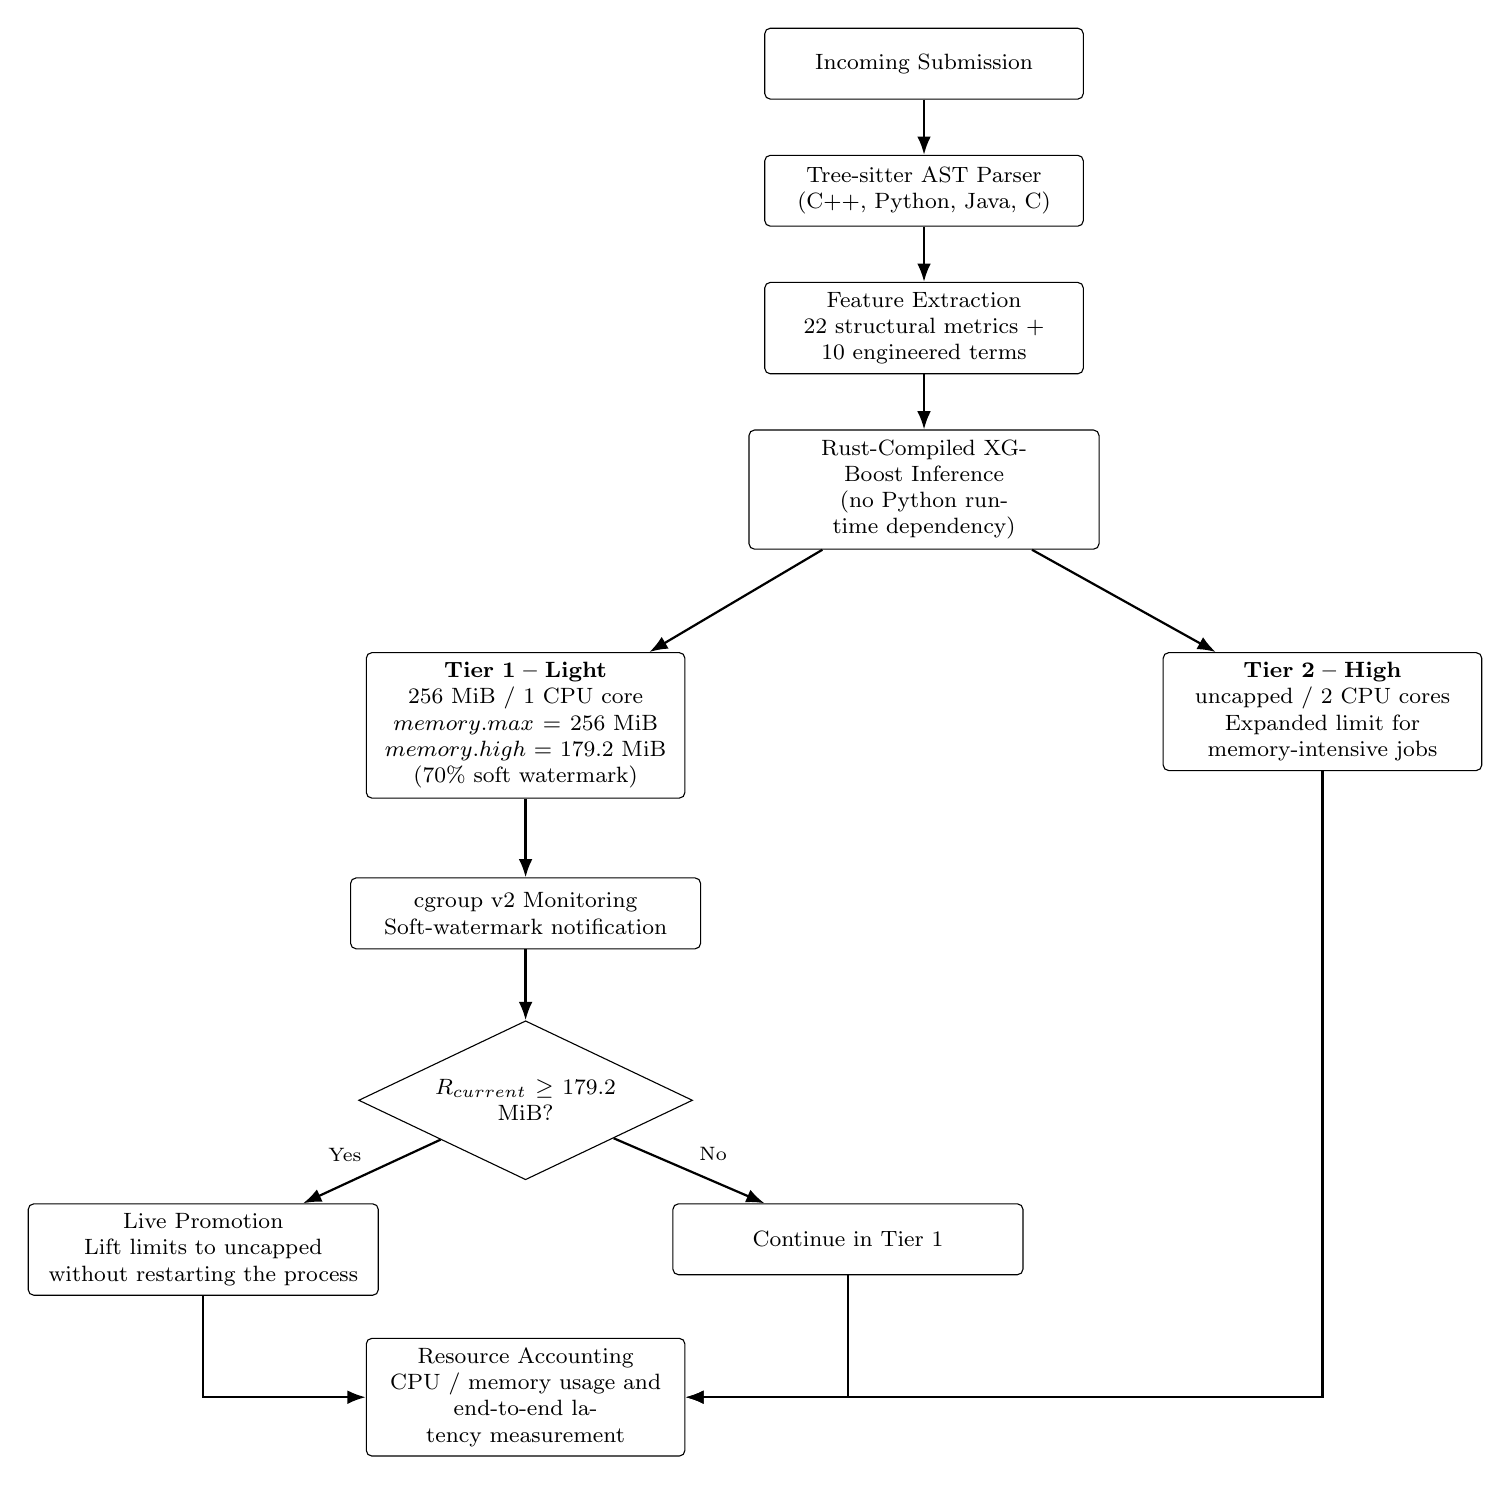
\begin{tikzpicture}[
    >=Latex,
    node distance=7mm and 16mm,
    block/.style={draw, rounded corners=2pt, align=center, minimum height=9mm, text width=38mm, inner sep=3.5pt, font=\footnotesize},
    smallblock/.style={draw, rounded corners=2pt, align=center, minimum height=9mm, text width=42mm, inner sep=3.5pt, font=\footnotesize},
    decision/.style={draw, diamond, aspect=2.1, align=center, inner sep=2pt, text width=27mm, font=\footnotesize},
    line/.style={-Latex, thick}
]
% Main processing pipeline: vertically stacked for a cleaner reading order.
\node[block] (input) {Incoming Submission};
\node[block, below=of input] (parser) {Tree-sitter AST Parser\\(C++, Python, Java, C)};
\node[block, below=of parser] (features) {Feature Extraction\\22 structural metrics +\\10 engineered terms};
\node[smallblock, below=of features] (model) {Rust-Compiled XGBoost Inference\\(no Python runtime dependency)};

% Initial resource tiers.
\node[block, below left=13mm and 8mm of model] (light) {\textbf{Tier 1 -- Light}\\256 MiB / 1 CPU core\\$memory.max=256$ MiB\\$memory.high=179.2$ MiB\\(70\% soft watermark)};
\node[block, below right=13mm and 8mm of model] (heavy) {\textbf{Tier 2 -- High}\\uncapped / 2 CPU cores\\Expanded limit for memory-intensive jobs};

% Reactive Tier 1 path.
\node[smallblock, below=10mm of light] (monitor) {cgroup v2 Monitoring\\Soft-watermark notification};
\node[decision, below=9mm of monitor] (decision) {$R_{current} \ge 179.2$ MiB?};
\node[smallblock, below left=8mm and 8mm of decision] (promote) {Live Promotion\\Lift limits to uncapped\\without restarting the process};
\node[smallblock, below right=8mm and 8mm of decision] (continue) {Continue in Tier 1};

% Final measurement stage centered beneath both branches.
\node[block, below=20mm of decision] (account) {Resource Accounting\\CPU / memory usage and\\end-to-end latency measurement};

% Main arrows.
\draw[line] (input) -- (parser);
\draw[line] (parser) -- (features);
\draw[line] (features) -- (model);
\draw[line] (model) -- (light);
\draw[line] (model) -- (heavy);
\draw[line] (light) -- (monitor);
\draw[line] (monitor) -- (decision);
\draw[line] (decision) -- node[above left, font=\scriptsize]{Yes} (promote);
\draw[line] (decision) -- node[above right, font=\scriptsize]{No} (continue);

% Cleanly route all execution paths into resource accounting.
\draw[line] (promote.south) |- (account.west);
\draw[line] (continue.south) |- (account.east);
\draw[line] (heavy.south) |- (account.east);

\end{tikzpicture}%
}
\caption{RAAS-OCJS execution and predictive tiering workflow. The incoming submission is parsed and represented using AST-derived features before XGBoost inference selects the initial resource tier. Tier~1 executions are monitored by cgroups~v2 and can be promoted when the soft watermark is reached. Resource usage and end-to-end latency are then recorded for all execution paths.}
\label{fig:raas_architecture}
\end{figure*}

\section{System Implementation and Methodology}

% MOVED TABLE: Placed here so it renders in Section IV


The evaluation testbed was implemented and calibrated on dedicated bare-metal hardware:
\begin{itemize}
    \item \textbf{Processor}: 13th Gen Intel Core i5-13420H (12 logical CPUs, 8 cores: 4 Performance cores up to 4.60 GHz + 4 Efficient cores up to 3.40 GHz).
    \item \textbf{Physical Memory}: 15 GiB usable DDR5 RAM.
    \item \textbf{Storage}: NVMe PCIe 4.0 Solid State Drive.
    \item \textbf{Operating System}: Fedora Linux (Kernel \texttt{7.1.3-201.fc44.x86\_64}).
    \item \textbf{Container Engine}: Docker Engine 29.8.1 with cgroupfs driver on unified hierarchy (\texttt{/sys/fs/cgroup}).
\end{itemize}



\subsection{Real Dataset Selection}
We measured real, ground-truth execution profiles by running 72 live container evaluations across four languages: C++20 (\texttt{g++ 14.2}), Python 3.12, Java 17 (OpenJDK HotSpot), and C17 (\texttt{gcc 14.2}). Benchmark problems were drawn from the Hugging Face \texttt{deepmind/code\_contests} \cite{li2022alphacode} and \texttt{CodeNet} \cite{puri2021codenet} datasets. These 72 measured profiles are what we sample from when driving the 10,000-submission and 500-submission simulations in Section~IV; those larger scenarios were not executed as 10,000 or 500 separate live container runs. Because CodeContests is crowd-sourced, we do not take the first solution offered for a language: each candidate is first executed against the problem's own public test, and only the first candidate returning \texttt{AC} is kept. Without this screening, two of the 72 cells failed for reasons unrelated to scheduling --- a non-compiling Java submission and a Python submission computing the wrong answer, each failing identically under all four strategies. 69 of the 72 runs return \texttt{AC} at the shipped 256~MiB tier; the three exceptions are Java on the memory-heavy problem, identified in Section~\ref{sec:boundary}.

Table~\ref{tab:mem_dist} gives the distribution this measurement rests on. The mean of 49.2~MiB is not representative of a typical submission and should be read with care: the median is 13.4~MiB. Four memory-heavy cells, all of them the two-dimensional knapsack problem, peak at 204--254~MiB and pull the mean roughly four times above the median. The distribution is bimodal rather than merely skewed --- most submissions sit an order of magnitude below the ceiling while a small number exhaust it --- and summarising it with a single mean conceals exactly the spread that motivates adaptive tiering.

\begin{table}[!t]
\caption{Resident Memory Used by the 69 Submissions Returning AC at the Shipped 256 MiB Tier}
\label{tab:mem_dist}
\centering
\small
\begin{tabular}{|l|c|c|c|c|c|}
\hline
\textbf{Language} & \textbf{Runs} & \textbf{$<$25 MiB} & \textbf{Median} & \textbf{Mean} & \textbf{Max} \\
\hline
C & 12 & 66.7\% & 19.3 MB & 72.3 MB & 204.8 MB \\
\hline
C++ & 20 & 80.0\% & 6.6 MB & 44.7 MB & 204.6 MB \\
\hline
Python & 20 & 80.0\% & 10.5 MB & 50.4 MB & 221.6 MB \\
\hline
Java & 17 & 76.5\% & 23.9 MB & 36.8 MB & 253.7 MB \\
\hline
\textbf{All} & \textbf{69} & \textbf{76.8\%} & \textbf{13.4 MB} & \textbf{49.2 MB} & \textbf{253.7 MB} \\
\hline
\end{tabular}
\end{table}



\subsection{AST Feature Extraction and XGBoost Predictive Tiering}
Before launching an execution container, RAAS-OCJS can optionally run a static code analysis pass to predict whether an incoming submission fits safely within Tier~1 (256~MiB) or should be provisioned directly with Tier~2 (uncapped). This predictive stage couples a Tree-sitter Abstract Syntax Tree (AST) feature extractor with in-process XGBoost classifiers \cite{chen2016xgboost}.

\textit{1) Static AST Feature Extraction:} Using language-specific Tree-sitter grammars compiled directly into our Rust daemon, the extractor parses source code into a concrete syntax tree in under 1.5~ms. In a single linear traversal of the tree, it computes 22 structural metrics:
\begin{itemize}
    \item \textbf{Control Flow and Loops}: Maximum block nesting depth, deepest loop nesting depth (which correlates with polynomial execution complexity $O(N^k)$), total loop statements, and McCabe cyclomatic complexity.
    \item \textbf{Recursion Topology}: A binary recursion flag and self-call site count, which differentiate simple linear recursion $O(N)$ from exponential divide-and-conquer or backtracking branching $O(2^N)$.
    \item \textbf{Memory and Container Patterns}: Detection of explicit large heap/BSS allocations ($\ge 10^6$ elements or bytes, such as \texttt{malloc}, \texttt{new int[]}, container sizing, or large static arrays), high-throughput I/O patterns (\texttt{sync\_with\_stdio}, \texttt{BufferedReader}, \texttt{sys.stdin.readline}), and standard library collections known for memory overhead (\texttt{unordered\_map}, \texttt{priority\_queue}, \texttt{BigInteger}, \texttt{defaultdict}).
    \item \textbf{Scale and Access Topology}: Total array/collection subscript expressions (\texttt{a[i]}), chained multi-dimensional indexing (\texttt{grid[i][j]} for 2D dynamic programming tables or graph adjacency matrices), function count, call sites, total AST node count, maximum tree depth, and source lines of code (SLOC).
\end{itemize}
From these 22 raw counts, the pipeline derives 10 interaction and scale terms: four density ratios normalised by AST size, source length, or function count (loop, call, subscript, and arithmetic density), a 2D subscript ratio, a recursion-intensity term, a log-scaled maximum integer constant --- which is what captures the literal size of an explicit allocation such as \texttt{new byte[200 << 20]} --- and log-scaled AST node and source character counts. This yields a 32-dimensional vector for the specialized per-language models, or 36 features for the unified model, which appends four one-hot language encodings.

\textit{2) Model Training and Validation:}
We trained gradient-boosted decision trees using XGBoost (\texttt{tree\_method='hist'}, learning rate $\eta = 0.05$, max tree depth $d = 6$, subsample ratio $0.8$, column subsample $0.8$, $L_1$ penalty $\alpha = 0.05$, and $L_2$ penalty $\lambda = 1.0$). Because contest submissions are heavily skewed toward lightweight solutions, we applied class re-weighting using $\texttt{scale\_pos\_weight} = N_{\mathrm{light}} / N_{\mathrm{heavy}}$ during training.

To avoid data leakage across submissions for the same problem, we evaluated the models with 5-fold \textbf{Problem-Grouped Cross-Validation} (\texttt{GroupKFold} grouped strictly by \texttt{problem\_id}). Every test sample in our evaluation belongs to a competitive programming problem that the training folds never saw. In addition, rather than accepting a default $0.5$ decision threshold, we tuned the threshold $\tau$ for each language using Youden's $J$ statistic ($J = \mathrm{Sensitivity} + \mathrm{Specificity} - 1$) on validation folds to balance recall against false tier promotions.

\begin{table*}[!t]
\caption{XGBoost Model Performance on Unseen Contest Problems (Problem-Grouped Validation)}
\label{tab:ml_metrics}
\centering
\small
\begin{tabularx}{\textwidth}{|Y|Y|c|c|c|c|c|c|}
\hline
\textbf{Dataset Source} & \textbf{Model Architecture} & \shortstack{\textbf{5-Fold}\\\textbf{CV Acc.}} & \shortstack{\textbf{Test Acc.}\\\textbf{(Unseen)}} & \textbf{F1-Score} & \textbf{Precision} & \textbf{Recall} & \shortstack{\textbf{ROC-}\\\textbf{AUC}} \\
\hline
IBM Project CodeNet & Specialized C++ Model & 87.32\% & 90.01\% & 90.91\% & 88.54\% & 93.41\% & 0.9612 \\
(71,218 Submissions) & Specialized C Model & 89.27\% & 89.26\% & 68.82\% & 55.98\% & 89.31\% & 0.9575 \\
& Specialized Python Model & 76.97\% & 79.45\% & 82.01\% & 80.33\% & 83.76\% & 0.8740 \\
& Specialized Java Model & 79.30\% & 78.20\% & 81.54\% & 82.03\% & 81.06\% & 0.8537 \\
& Unified Multi-Language & 82.19\% & 83.71\% & 84.81\% & 80.19\% & 89.99\% & 0.9149 \\
\hline
DeepMind CodeContests & Unified Multi-Language & 86.74\% & 86.78\% & 89.64\% & 82.74\% & 97.79\% & 0.9606 \\
(30,000 Submissions) & Specialized Python Model & 95.76\% & 98.88\% & 99.41\% & 98.82\% & 100.0\% & 0.9812 \\
& Specialized C++ Model & 84.27\% & 83.94\% & 87.49\% & 78.67\% & 98.53\% & 0.9474 \\
& Specialized Java Model & 79.43\% & 82.32\% & 83.28\% & 73.09\% & 96.76\% & 0.9430 \\
\hline
\end{tabularx}
\end{table*}

\textit{3) Empirical Model Metrics on Unseen Problems:}
Table~\ref{tab:ml_metrics} summarizes performance on held-out, unseen contest problems across both IBM Project CodeNet (71,218 submissions) and DeepMind CodeContests (30,000 submissions). On CodeNet, the specialized C++ model reached a 90.01\% test accuracy, a 90.91\% F1-score, and an ROC-AUC of 0.9612 on unseen problems. The specialized Python and Java models achieved 79.45\% and 78.20\% test accuracy (ROC-AUC of 0.8740 and 0.8537, respectively). On DeepMind CodeContests, where problems feature diverse algorithmic structures from Codeforces and HackerEarth, the specialized models scored up to 98.88\% test accuracy in Python and 83.94\% in C++ (Table~\ref{tab:ml_metrics}).

\textit{4) In-Process Rust Inference:}
To avoid running a Python interpreter or querying an external model-serving daemon during the latency-critical judging loop, we compiled the trained XGBoost decision trees directly into native Rust source files (\texttt{server/src/generated/*.rs}) using \texttt{m2cgen}. These functions compile straight into the judge binary. At execution time the XGBoost tree evaluation itself takes under $10\ \mu\text{s}$. That figure is \emph{not} the cost of Stage~2 as a whole: Stage~2 in Table~\ref{tab:e2e_latency} is \emph{AST parse and Tree-sitter prediction combined}, and totals 0.89--1.45~ms, of which tree evaluation is a negligible part. The AST parse dominates that stage.

\textit{5) Role in Scheduling Strategies:}
In RAAS-OCJS, predictive classification can be used on its own or paired with the kernel watermark. Under the \textbf{Predictive} strategy, a submission with $P(\mathrm{Heavy}) \ge \tau_{\mathrm{lang}}$ starts directly in Tier~2. Under the \textbf{Hybrid} strategy, the model provides the initial tier choice, but the cgroups~v2 soft watermark ($\theta = 70\%$, 179.2~MiB) remains active in the background: if a heavy submission is mistakenly started in Tier~1, the kernel watermark trips and promotes the container mid-execution, preventing an Out-Of-Memory abort despite the misprediction. Section~\ref{sec:classifier_eval} quantifies the misrouting rate that makes this guarantee necessary: the classifier alone cannot supply it.

\subsection{End-to-End Latency Pipeline Breakdown}
To ensure transparent latency accounting, RAAS-OCJS instrumented every submission across 7 discrete stages:
\begin{equation}
\begin{aligned}
T_{\mathrm{e2e}} ={}&
T_{\mathrm{net\_in}} + T_{\mathrm{parse}} +
T_{\mathrm{queue}} + T_{\mathrm{init}} \\
&+ T_{\mathrm{comp}} + T_{\mathrm{exec}} +
T_{\mathrm{tear}} + T_{\mathrm{net\_out}}
\end{aligned}
\end{equation}

\begin{table*}[htbp]
\caption{End-to-End Verdict Pipeline Latency Breakdown (Milliseconds)}
\label{tab:e2e_latency}
\begin{center}
\begin{tabular}{|c|c|c|c|c|}
\hline
\textbf{Pipeline Stage} & \textbf{C++ (g++)} & \textbf{Python (3.12)} & \textbf{Java (OpenJDK 17)} & \textbf{C (gcc)} \\
\hline
1. Network Inbound Ingestion & 0.38 ms & 0.38 ms & 0.38 ms & 0.38 ms \\
\hline
2. AST Parse \& Tree-sitter Predict & 1.12 ms & 0.89 ms & 1.45 ms & 0.94 ms \\
\hline
3. Queue Scheduling \& Dispatch & 0.08 ms & 0.08 ms & 0.08 ms & 0.08 ms \\
\hline
4. Container Sandbox Initialization & 18.42 ms & 17.91 ms & 19.20 ms & 18.15 ms \\
\hline
5. Compilation / Bytecode Translation & 312.45 ms & N/A (Interpreted) & 842.10 ms & 284.12 ms \\
\hline
6. In-Sandbox Test Execution & 48.12 ms & 74.50 ms & 112.40 ms & 45.20 ms \\
\hline
7. Container Teardown \& Result Egress & 12.45 ms & 11.80 ms & 13.25 ms & 12.10 ms \\
\hline
\textbf{Total Turnaround Latency (E2E)} & \textbf{393.00 ms} & \textbf{105.56 ms} & \textbf{988.86 ms} & \textbf{360.97 ms} \\
\hline
\end{tabular}
\end{center}
\end{table*}

\section{Empirical Results and Macro Contest Simulation}

% MOVED TABLE: Placed here so it renders in Section V or VI
\begin{table*}[!t]
\caption{Outcome of the Full 72-Run Benchmark at a 128 MiB Tier}
\label{tab:128mb_boundary}
\centering
\small
\begin{tabularx}{\textwidth}{|c|c|c|c|c|c|Y|}
\hline
\textbf{Language} & \textbf{Runs} & \textbf{AC} & \textbf{SE} & \textbf{MLE} & \textbf{RE} & \textbf{Dominant Failure} \\
\hline
C & 12 & 9 & 0 & 2 & 1 & Knapsack outgrows the tier \\
\hline
C++ & 20 & 9 & \textbf{8} & 3 & 0 & \textbf{Will not compile: g++ needs 189--211 MB} \\
\hline
Python & 20 & 17 & 0 & 2 & 1 & Knapsack outgrows the tier \\
\hline
Java & 20 & 17 & 0 & 2 & 1 & Knapsack outgrows the tier \\
\hline
\textbf{Total} & \textbf{72} & \textbf{52} & \textbf{8} & \textbf{9} & \textbf{3} & --- \\
\hline
\end{tabularx}
\end{table*}


\subsection{Classifier Routing Accuracy on the Benchmark Corpus}
\label{sec:classifier_eval}
The classifier is evaluated here against ground truth on the six-problem corpus, because this is the distribution the judge actually serves. Only the two-dimensional knapsack across the four languages is genuinely memory-heavy, giving 4 heavy cells against 14 light ones.

\begin{table}[!t]
\caption{Classifier Routing Against Ground Truth on the 18 Benchmark Programs}
\label{tab:classifier_routing}
\centering
\small
\begin{tabular}{|l|c|c|}
\hline
& \textbf{Predicted Heavy} & \textbf{Predicted Light} \\
\hline
\textbf{Truly Heavy} (4 cells) & 0 & 4 \\
\hline
\textbf{Truly Light} (14 cells) & 8 & 6 \\
\hline
\end{tabular}
\end{table}

This gives a routing accuracy of 33.3\% (6 of 18). A constant \emph{light} prediction would score 77.8\% (14 of 18) on the same corpus, so on this distribution the classifier performs worse than a trivial strategy: it misses every genuinely heavy cell and raises eight false alarms. We verified the routing independently of the measurement harness by submitting single-purpose probes directly to the API; a program peaking at 206~MB through bulk buffer allocation is routed \emph{light}, while one peaking at 9.6~MB through collection churn is routed \emph{heavy}, confirming the direction of the error.

This is a distribution-shift result rather than a statement about the model's quality in general: the same unified model reaches 83.71\% held-out accuracy on unseen CodeNet problems (Table~\ref{tab:ml_metrics}). The corpus is small --- six problems --- and its heavy class is under-represented. The finding nonetheless bears directly on the design, because a system whose memory safety rested on this classifier would route heavy submissions into the bounded tier and rely on nothing else to catch them.

\subsection{Macro-Scale 10,000 Contest Simulation}
To estimate resource savings across a full-scale contest, we ran a discrete-event simulation of 10,000 submissions, sampling resource-usage profiles from our 72 measured runs and assigning a language distribution of 40\% C++, 35\% Python, 15\% Java, and 10\% C. This is a simulation seeded with real measurements, not a live execution of 10,000 submissions. Reservation is charged from the judge's own tier decision for each submission: a bounded-tier start costs the tier size, and an uncapped start or a mid-execution promotion is charged the 2048~MiB baseline ceiling as a worst case.

Table~\ref{tab:macro_sim} reports the Reactive strategy, which was the most efficient measured. Two results were not anticipated. First, Reactive reserves less than every other strategy, including Hybrid: Hybrid pre-assigns each submission its classifier labels heavy to an uncapped container, and such a container carries no reserved capacity, so it must be charged at the worst-case ceiling, reaching only 22.45\%. Prediction alone reaches 40.23\%. Because Hybrid and Predictive share one classifier for the initial tier, they start the identical set of submissions uncapped, and promotion can only raise a reservation and never lower it. Prediction is not free --- it costs reservation, and on this corpus it costs more than it saves. Second, no strategy changes steady-state latency: P95 turnaround spans 1,185.86--1,192.01~ms across all four, a spread inside run-to-run noise. The saving is free in latency terms, but it is not a latency improvement.

\begin{table}[!t]
\caption{Macro-Scale 10,000 Submission Contest Simulation (256 MiB Tier)}
\label{tab:macro_sim}
\centering
\small
\begin{tabular}{|P{2.4cm}|c|c|P{1.6cm}|}
\hline
\textbf{Performance Metric} & \textbf{Static (2048 MiB)} & \textbf{Reactive} & \textbf{Reduction} \\
\hline
Total Submissions & 10,000 & 10,000 & --- \\
\hline
Total RAM Reserved & 20,000.00 GB & 10,557.00 GB & \textbf{47.22\%} \\
\hline
Peak Memory Actually Used & 505.50 GB & 447.45 GB & 11.5\% \\
\hline
Allocated Memory Wasted & 97.47\% & 95.76\% & 1.71 pp \\
\hline
Live Promotions & --- & 2,032 (20.3\%) & n/a \\
\hline
Total CPU Core-Hours & 4.337 hrs & 3.379 hrs & \textbf{22.09\%} \\
\hline
P95 Turnaround (steady state) & 1,187.00 ms & 1,185.86 ms & negligible \\
\hline
\end{tabular}
\end{table}

\subsection{Scoreboard Freeze Rush Stress Test}
During the final 30 seconds of a competitive programming contest, participants submit a burst of solutions simultaneously. We modeled a 500-submission flash burst using the profiles measured on our bare-metal host, run through the same simulation as Section~IV-B rather than as a live 500-submission run.

\begin{table}[!t]
\caption{500-Submission Freeze Rush Stress Test (15 GiB Host, 256 MiB Tier)}
\label{tab:burst_stress}
\centering
\small
\begin{tabularx}{\columnwidth}{|Y|c|c|Y|}
\hline
\textbf{Throughput Metric} & \textbf{Static Baseline} & \textbf{Reactive} & \textbf{Improvement} \\
\hline
Concurrent Slots & 7 & 56 & 8.0$\times$ expansion \\
\hline
Avg Queue Wait & 12,386.2 ms & 0.0 ms & \textbf{100\% eliminated} \\
\hline
P95 Queue Wait & 23,847.2 ms & 0.0 ms & \textbf{100\% eliminated} \\
\hline
P95 Turnaround & 24,918.4 ms & 1,186.8 ms & \textbf{21.0$\times$} \\
\hline
Burst Drain Time & 56.5 s & 31.2 s & 25.3 s faster \\
\hline
\end{tabularx}
\end{table}

As shown in Table~\ref{tab:burst_stress}, the static baseline causes severe queue congestion, with an average wait of 12.4 seconds and a 56.5 second drain that leaves jobs completing after the contest deadline. RAAS-OCJS expands safe concurrency to 56 slots, driving queue wait to \textbf{0.0~ms} and completing the entire burst within 31.2 seconds. Note that the gain here comes from admitting more concurrent slots, not from finishing individual submissions faster: steady-state P95 turnaround is 1,187.00~ms under the static baseline and 1,185.86~ms under Reactive, a difference well within run-to-run noise. Overcommitting the baseline to 14 slots does recover most of the wait (250.4~ms) and also drains in 31.6~s, but at 186\% host memory utilisation, which is precisely the failure mode the tiered scheduler avoids.

\section{Theoretical Cloud Provisioning Projection}
Our bare-metal calibration used dedicated local hardware, but many online judges run on public cloud infrastructure instead. To estimate the effect there, we built a theoretical projection mapping our measured kernel profiles onto an AWS EC2 cluster of \texttt{c6i.4xlarge} instances (16 vCPUs, 32~GB RAM @ USD 0.68 per hour). These figures depend on the pricing and instance-type assumptions stated here and should be read as a projection, not a deployed cloud measurement.

Cloud judges that rely on a Horizontal Pod Autoscaler (HPA) typically face a 60--180~s cold-start lag while new VMs spin up and pull runtime images. Because RAAS-OCJS's lighter default tier packs more submissions per existing VM, our projection shows the initial VM fleet absorbing a flash rush in place.

Every figure in Table~\ref{tab:cloud} is derived from the shipped 256~MiB tier, the instance size, and the hourly price rather than transcribed, and assumes 87.5\% host utilisation when packing pods --- the same packing ceiling the static baseline achieves (14 pods $\times$ 2048~MiB of 32~GB).

\begin{table}[!t]
\caption{AWS Provisioning Projection at the Shipped 256 MiB Tier}
\label{tab:cloud}
\centering
\small
\begin{tabular}{|P{4.2cm}|c|c|c|}
\hline
\textbf{Provisioning Dimension} & \textbf{Baseline} & \textbf{RAAS-OCJS} & \textbf{Gain} \\
\hline
Per-Pod Memory & 2048 MiB & 256 MiB & \textbf{8.0$\times$} \\
\hline
Per-Pod CPU & 2.0 vCPU & 1.0 vCPU & 2.0$\times$ \\
\hline
Pods per VM & 14 & 112 & \textbf{8.0$\times$} \\
\hline
VMs for 500-Sub Burst & 36 & 5 & \textbf{86.1\% fewer} \\
\hline
Cluster Hourly Cost & USD 24.48 & USD 3.40 & \textbf{USD 21.08} \\
\hline
10k RAM Reserved & 20,000.00 GB & 10,557.00 GB & \textbf{47.22\%} \\
\hline
\end{tabular}
\end{table}

The projected hourly saving is \textbf{USD~21.08}, an 86.1\% reduction in cluster cost.

\section{Boundary Stress Analysis and Future Scopes}

\subsection{Squeezing Tier 1 to 128 MiB: What Sets the Floor}
\label{sec:boundary}
To locate the floor, we re-ran the full 72-run benchmark with Tier~1 set to \textbf{128~MiB} ($\theta = 70\%$, watermark $= 89.6$~MiB, leaving a 38.4~MiB buffer below the hard limit).

The tier fails, and the interesting result is that it fails for three independent reasons rather than one. 52 of 72 runs returned \texttt{AC}, against 69 of 72 at the shipped 256~MiB tier (Table~\ref{tab:128mb_boundary}).

\textbf{1. The C++ toolchain does not fit.} Eight runs returned a bare \texttt{SE} with no case results and zero CPU time, all of them C++: the container never produced a compiled binary. Measuring the compiler directly, \texttt{g++ -O2} peaks at 189--211~MB of resident memory on these sources (P1 189.4~MB, P2 190.9~MB, P3 198.2~MB, P4 210.8~MB). Compilation runs inside the submission container, so a 128~MiB tier cannot build them at all. This is a property of the tier, not of the scheduler: no strategy can rescue a submission that never compiled. The knapsack source compiles in 60.6~MB and so does reach execution, which is why C++ shows both \texttt{SE} and \texttt{MLE} rather than one or the other.

\textbf{2. The watermark window is too narrow.} Every knapsack cell failed in every language under every strategy, including Reactive and Hybrid, which did promote. Promotion completed at 253--794~ms, but the program crosses 128~MiB before it can land. The window between the watermark (89.6~MiB) and the hard limit is only 38.4~MiB, and these submissions allocate at a rate that consumes it well inside the promotion path's latency. At the 256~MiB tier the same window is 76.8~MiB and the mechanism holds for C, C++ and Python.

\textbf{3. The JVM heap allowance contradicts the container cap.} Java was the only language to fail at the shipped tier as well: three \texttt{MLE} verdicts at 256~MiB, in Predictive, Reactive and Hybrid alike, with peaks of 255--256~MB. The runtime is started with \texttt{-Xmx512m}, a 512~MB heap allowance, inside a 256~MiB container. The JVM grows its heap toward that allowance and crosses the container ceiling. The two limits are mutually inconsistent and should be reconciled by sizing \texttt{-Xmx} as a fraction of the tier, or by raising the tier for JVM workloads.

Taken together these set \textbf{256~MiB as the practical minimum Tier~1 limit}, but for reasons different from those we initially expected. The limit is not set by the classifier, and only partly by the promotion mechanism: it is set by the largest of three demands the tier must simultaneously satisfy --- the toolchain used to build the submission, the watermark window needed to promote it in time, and the runtime's own overhead above the program's working set.

\subsection{Future Research Scopes}
Based on these boundary observations, we outline five key future scopes:
\begin{enumerate}
    \item \textbf{Toolchain-Aware Tier Sizing}: A 128~MiB tier cannot compile C++ at all, since \texttt{g++} alone peaks at 189--211~MB, so tier selection must account for the build step and not only for the runtime. Measuring per-language build cost and provisioning the tier as $\max(\text{build}, \text{runtime})$ would let lighter languages run in a smaller tier without stranding compiled ones.
    \item \textbf{Watermark Tuning Against Allocation Rate}: The 38.4~MiB window at a 128~MiB tier is too narrow to outrun a submission needing twice the tier, whereas 76.8~MiB holds at 256~MiB. What matters is not the fraction but the absolute window relative to how fast a submission claims memory, which argues for sizing the watermark from a measured allocation rate rather than a fixed percentage.
    \item \textbf{Reconciling \texttt{-Xmx} with the Tier}: The runtime is configured with a 512~MB heap allowance inside a 256~MiB container, which cannot be honoured. Sizing \texttt{-Xmx} below the tier, and pairing it with an allocator that grows heap in smaller increments such as \texttt{-XX:+UseSerialGC}, would remove the contradiction we measured.
    \item \textbf{Deliberate, Bounded Swap}: We disabled swap because Docker's default was silently doubling the tier and invalidating our measurements. A small, explicitly sized allowance (e.g. \texttt{--memory-swap} 25\% above \texttt{--memory}) could absorb the allocation spikes that occur during promotion, provided the tier's real ceiling is stated rather than left to a default.
    \item \textbf{Hardware-Level MicroVM Isolation}: Integrating Firecracker or gVisor to provide kernel-level security hardening for the Heavy execution tier.
\end{enumerate}

\section{Conclusion}
Fixed, worst-case resource limits reduce how many submissions an online judge can run concurrently, and that effect is most visible on fixed physical hardware where more machines cannot simply be added. In our simulations, seeded with real measured profiles, the two-tier RAAS-OCJS configuration reclaimed 47.22\% of reserved memory (10,557.00 GB of 20,000) and cut CPU core-hours by 22.09\% relative to a static 2048~MiB baseline. The simulated 500-submission burst showed average queue wait dropping from 12,386.2~ms to 0.0~ms, with a correspondingly shorter contest clear time.

Three findings temper the result, and we consider all three load-bearing rather than incidental.

First, prediction did not pay for itself on this corpus. Routing by the classifier alone reached 40.23\%, and prediction combined with the watermark reached only 22.45\%, because a container the classifier marks heavy is left uncapped and therefore carries no reserved capacity to count as saving. Since the two strategies share one classifier for the initial tier and promotion can only raise a reservation, Hybrid can never reserve less than Predictive: it pays for the classifier's false alarms and still needs the watermark. Reactive promotion --- start bounded, escalate on evidence --- was the most efficient strategy measured, at 47.22\%. That the mechanism outperforms the predictor is the paper's more defensible claim, and it points to classifier reuse rather than classifier reliance as the design direction.

Second, the classifier is weak outside its training distribution. It routes 33.3\% of submissions correctly on our six-problem corpus, below the 77.8\% a constant \emph{light} prediction would score (Table~\ref{tab:classifier_routing}), despite reaching 83.71\% held-out accuracy on unseen CodeNet problems. A system whose resource safety depended on that classifier would be fragile; the watermark does not depend on it, which is what makes a bounded-tier start safe to deploy.

Third, our attempt to locate the floor by squeezing Tier~1 to 128~MiB failed for three independent reasons, and we report that failure rather than a tidier positive result, because it is what establishes the floor. The C++ toolchain alone needs 189--211~MB and cannot build a submission inside the tier; the 38.4~MiB watermark window is too narrow to promote a submission that outgrows the tier, so every strategy lost the memory-heavy problem; and the JVM is configured with a heap allowance twice the size of its container, an inconsistency that surfaces as \texttt{MLE} at 256~MiB as well. The tier must therefore simultaneously accommodate the build step, the watermark window needed for timely promotion, and the runtime's overhead above the program's working set. It is the largest of those three, not the classifier, that sets 256~MiB as the practical minimum.

Taken together, these results indicate that adaptive resource allocation is a practical direction for online code judge infrastructure, with the watermark rather than the classifier as its load-bearing component. The cloud cost figures remain a projection, and the approach still needs testing against a wider range of real, larger-scale workloads.

\bibliographystyle{IEEEtran}
\begin{thebibliography}{00}
\bibitem{song2025idl} L. Song, Y. Han, Y. Guo, and C. Cai, ``IDL-LTSOJ: Research and implementation of an intelligent online judge system utilizing DNN for defect localization,'' \textit{High-Confidence Computing}, vol. 5, no. 2, p. 100268, 2025.
\bibitem{pan2022cloud} G.-C. Pan, P. Liu, and J.-J. Wu, ``A cloud-native online judge system,'' in \textit{Proc. IEEE 46th Annu. Computers, Software, and Applications Conf. (COMPSAC)}, 2022, pp. 1293--1298.
\bibitem{zhang2024intelligent} E. Zhang, F. Wu, and X. Lu, ``An intelligent scheduling system for large-scale online judging,'' in \textit{Computer Science and Education. Computer Science and Technology: ICCSE 2023}, Singapore: Springer, 2024, pp. 265--279.
\bibitem{wasik2018survey} S. Wasik, M. Antczak, J. Badura, A. Laskowski, and T. Sternal, ``A survey on online judge systems and their applications,'' \textit{ACM Computing Surveys}, vol. 51, no. 1, pp. 1--34, 2018.
\bibitem{wang2021metaoj} M. Wang, W. Han, and W. Chen, ``MetaOJ: A massive distributed online judge system,'' \textit{Tsinghua Science and Technology}, vol. 26, no. 4, pp. 548--557, 2021.
\bibitem{puri2021codenet} R. Puri et al., ``Project CodeNet: A large-scale AI for code dataset for learning a diversity of coding tasks,'' in \textit{Proc. Neural Information Processing Systems (NeurIPS) Datasets and Benchmarks Track}, 2021.
\bibitem{li2022alphacode} Y. Li et al., ``Competition-level code generation with AlphaCode,'' \textit{Science}, vol. 378, no. 6624, pp. 1092--1097, 2022.
\bibitem{cgroups2024} Linux Kernel Organization, ``Control Group v2 Specification,'' kernel.org documentation, 2024. [Online]. Available: \url{https://docs.kernel.org/admin-guide/cgroup-v2.html}
\bibitem{chen2016xgboost} T. Chen and C. Guestrin, ``XGBoost: A scalable tree boosting system,'' in \textit{Proc. 22nd ACM SIGKDD Int. Conf. Knowledge Discovery and Data Mining (KDD)}, 2016, pp. 785--794.
\end{thebibliography}

\end{document}